\documentclass[conference]{IEEEtran}
%\documentclass[conference, onecolumn]{IEEEtran}
%\documentclass[10pt,twocolumn]{article} 
%\usepackage{latex8}
%\usepackage{times}

%\renewcommand\thesection{\arabic{section}}
%\renewcommand\thesubsection{\thesection.\arabic{subsection}}
%\renewcommand\thesubsubsection{\thesubsection.\arabic{subsubsection}}

%\renewcommand\thesectiondis{\arabic{section}}
%\renewcommand\thesubsectiondis{\thesectiondis.\arabic{subsection}}
%\renewcommand\thesubsubsectiondis{\thesubsectiondis.\arabic{subsubsection}}



\usepackage[pdftex]{graphicx}
\usepackage{epsfig}
\usepackage{amsmath,amssymb,amsthm}
\usepackage{subfig}
\usepackage{cite}

\usepackage{tikz}

%\usepackage{etoolbox}

\usepackage{color}

\newcommand{\ceiling}[1]{\left\lceil{#1}\right\rceil}
\newcommand{\floor}[1]{\left\lfloor{#1}\right\rfloor}
\newcommand{\setof}[1]{\left\{{#1}\right\}}
\newcommand{\set}[2]{\{{#1}\mid{#2}\}}
\newcommand{\equals}{\stackrel{\mathrm{def}}{=}}

\newcommand{\jj}[1]{\textcolor{blue}{jj: #1 : endjj}}
\newcommand{\kh}[1]{\textcolor{magenta}{kevin: #1 : endkevin}}
\newcommand{\framework}[1]{$\mathbf{k^2U}$}
\newcommand{\frameworkkq}[1]{$\mathbf{k^2Q}$}
\newcommand{\Cong}[1]{\textcolor{red}{cong: #1 : endcong}}


%%%%%%%%%%%%%%%
 \def\myendproof{\qed}%{\ \vbox{\hrule\hbox{%
   %\vrule height1.3ex\hskip0.8ex\vrule}\hrule }}\par}
 %\renewenvironment{proof}{\noindent{\bf Proof. }}{\myendproof}
%%%%%%%%%%%%%%
%%%%%%%%%%%%%%%
 \newenvironment{appProof}[1]{\noindent{\bf Proof of
     #1. }}{\myendproof\vskip 0.1in}
 %%%%%%%%%%%%%%

\newtheorem{theorem}{Theorem}
\newtheorem{Lemma}{Lemma}
\newtheorem{Corollary}{Corollary}
\newtheorem{example}{Example}
\newtheorem{claim}{Claim}
\newtheorem{definition}{Definition}
\newtheorem{rrule}{Rule}
\newtheorem{remark}{Remark}
\newtheorem{observation}{Observation}
\newtheorem{Property}{Property}


\usetikzlibrary{%
  arrows,%
  shapes.misc,% wg. rounded rectangle
  shapes.arrows,%
  chains,%
  matrix,%
  positioning,% wg. " of "
  scopes,%
  decorations.pathmorphing,% /pgf/decoration/random steps | erste Graphik
  shadows%
}

\pgfdeclarelayer{background}
\pgfdeclarelayer{foreground}
\pgfsetlayers{background,main,foreground}
\tikzstyle{materia}=[draw, fill=white, text width=1.0em, text centered,
  minimum height=4em,drop shadow]
\tikzstyle{practica} = [materia, text width=18em, minimum width=8em,
align =left,
  minimum height=3em, rounded corners, drop shadow]
\tikzstyle{texto} = [above, text width=6em, text centered]
\tikzstyle{linepart} = [draw, thick, color=blue!50, -latex', dashed]
\tikzstyle{line} = [draw, line width = 2pt, color=blue!50, -latex']
\tikzstyle{ur}=[draw, text centered, minimum height=0.01em]

\bibliographystyle{abbrv} 

%\newif\ifpaper
%\paperfalse

\pagestyle{plain}

\begin{document}
  
\title{A Unifying Response Time Analysis Framework for Dynamic Self-Suspending Tasks}

\author{Jian-Jia Chen\IEEEauthorrefmark{1}, Geoffrey Nelissen\IEEEauthorrefmark{4}, Wen-Hung Huang\IEEEauthorrefmark{1}\\
\IEEEauthorrefmark{1} TU Dortmund University, Germany\\
\IEEEauthorrefmark{4} CISTER/INESC-TEC, ISEP, Polytechnic Institute of Porto, Portugal \\
Emails: \{jian-jia.chen, wen-hung.huang\}@tu-dortmund.de, grrpn@isep.ipp.pt
}

\maketitle

\begin{abstract}
  For real-time embedded systems, self-suspending behaviour can cause
  substantial performance/schedulability degradation. In this paper,
  we focus on preemptive fixed-priority scheduling for the dynamic
  self-suspension task model on a uniprocessor platform. In this
  model, a job of a sporadic task can suspend itself dynamically under
  a specified upper bound on the self-suspension across all of its
  suspension phases. To quantify the higher-priority interferences,
  the results in the literature for this task model can be classified
  into three classes (i) suspension as computation, (ii)
  suspension-induced release jitter, and (iii) suspension as blocking.
  However, the suspension-induced release jitter has to be carefully
  specified, and the concept to model suspension as blocking was never
  proven to be correct in the past. This paper presents a unifying
  response time analysis framework for the dynamic self-suspending
  task model. We provide a rigorous proof and show that all the three
  classes mentioned above are analytically dominated by this unifying
  framework. Therefore, all of them are in fact correct, and are
  inferior to the proposed response time analysis in this paper.  The
  evaluation results show that the analysis framework can have a huge
  improvement (an increase of up to $50\%$ of the number of task sets
  deemed schedulable) over these state-of-the-art analyses.
\end{abstract}

\section{Introduction}

The periodic/sporadic task model has been recognized as the basic
model for real-time systems with recurring executions.  A sporadic
real-time task $\tau_i$ is characterized by its \emph{worst-case execution
time} $C_i$, its \emph{minimum
  inter-arrival time} $T_i$ and its
\emph{relative deadline} $D_i$. A sporadic task defines an infinite
sequence of task instances, also called \emph{jobs}, that arrive with
the minimum inter-arrival time constraint. When a job of task $\tau_i$
arrives at time $t$, the job should finish no later than its
\emph{absolute deadline} $t+D_i$, and the next job of task $\tau_i$
can only be released no earlier than $t+T_i$. For the periodic task
model, the next job is released at time $t+T_i$. $T_i$ is
then also referred to as the \emph{period} of $\tau_i$.


The seminal work by Liu and Layland \cite{Liu_1973} considered the
scheduling of periodic tasks and presented the schedulability analyses
based on utilization bounds to verify whether the deadlines are met or
not.  For decades, researchers in real-time systems have
devoted themselves to effective design and efficient analyses of
different recurrent task models to ensure that tasks can meet their
specified deadlines. In most of these studies, \emph{a task usually does not
 suspend itself}. That is, after a job is released, the job
is either executed or stays in the ready queue, but it is not moved to
the suspension state.  Such an assumption is valid only under the
following conditions: (1) the latency of the memory accesses and I/O
peripherals is considered to be part of the worst-case execution time
of a job, (2) there is no external device for accelerating the
computation, and (3) there is no synchronization between different
tasks on different processors in a multiprocessor or distributed
computing platform.


If a job can suspend itself before it finishes its computation,
self-suspension behaviour has to be considered. Due to the interaction
with other system components and synchronization, self-suspension
behaviour has become more visible in designing real-time embedded
systems.  Typically, the resulting suspension delays range from a few
microseconds (e.g., a write operation on a flash
drive~\cite{Kang:rtss07}) to a few hundreds of milliseconds (e.g.,
offloading computation to GPUs~\cite{Kato_2011,Liu_2014}).

There are two typical models for self-suspending sporadic task
systems: 1) the dynamic self-suspension task model, and 2) the
segmented self-suspension task model. In the \emph{dynamic}
self-suspension task model, in addition to the worst-case execution time
$C_i$ of sporadic task $\tau_i$, we have also the worst-case
self-suspension time $S_i$ of task $\tau_i$. In the \emph{segmented} self-suspension
task model, the execution behaviour of a job of task $\tau_i$ is
specified by interleaved computation segments and self-suspension
intervals.  From the system designer's perspective, the dynamic
self-suspension model provides a simple specification by ignoring the
juncture of I/O access, computation offloading, or
synchronization. However, if the suspending behaviour can be
characterized by using a segmented pattern, the segmented
self-suspension task model can be more appropriate.

In this paper, we focus on preemptive fixed-priority scheduling for
the dynamic self-suspension task model on a uniprocessor platform. To
verify the schedulability of a given task set, this problem has been
specifically studied in
\cite{RTCSA-KimCPKH95,MingLiRTCSA1994,ECRTS-AudsleyB04,RTAS-AudsleyB04,huangpass:dac2015}.
The recent report by Chen et al.\footnote{The report, with a tentative
  title ``Many Suspensions, Many Problems: A Review of
  Self-Suspending Tasks in Real-Time Systems'' (all the authors in
  this paper are contributors to this review), has been
  finalized. However, it is under the final internal review by the
  co-authors.  We hope the report to be filed in the early March
  2016.} and the report by Bletsas et al. \cite{BletsasReport2015}
have shown that several analyses in the state-of-the-art of self-suspending tasks~\cite{ECRTS-AudsleyB04,RTAS-AudsleyB04,RTCSA-KimCPKH95,MingLiRTCSA1994}
are in fact unsafe. Unfortunately, those misconceptions propagated to several works~\cite{zeng-2011,bbb-2013,yang-2013,kim-2014,han-2014,carminati-2014,yang-2014,lakshmanan-2009}
analyzing the worst-case response time for partitioned multiprocessor
real-time locking protocols.

Furthermore, one of the seminal result presented by Jane W. S. Liu in her book titled "Real-Time Systems"
\cite[p. 164-165]{Liu:2000:RS:518501} and implicitly used
by Rajkumar, Sha, and Lehoczky \cite[p.
267]{DBLP:conf/rtss/RajkumarSL88} for analyzing the self-suspending
behaviour due to synchronization protocols in multiprocessor systems, was never proven correct.
%However, there is no proof in
%\cite{Liu:2000:RS:518501,DBLP:conf/rtss/RajkumarSL88} to support the
%correctness of the provided schedulability tests.

\noindent\textbf{Contributions.} In this paper, we propose the following contributions:
\begin{compactitem}
\item We provide a new response analysis framework for dynamic self-suspending
  sporadic real-time tasks executing on a uniprocessor platform. The
  key observation in our analysis is that the \emph{interference from higher-priority
    self-suspending tasks can be arbitrarily modelled as jitter or
    carry-in terms}.
\item We prove that the new analysis analytically
  dominates all the existing results in the state-of-the-art, excluding the flawed ones.  
\item We prove the
  correctness of the analysis initially proposed in \cite[p.
  164-165]{Liu:2000:RS:518501} and
  \cite[p. 267]{DBLP:conf/rtss/RajkumarSL88}, which were never proven correct in the state-of-the-art\footnote{A simplified
    version of the proof of Theorem~\ref{theorem:general-framework} to support the correctness of \cite[p. 164-165]{Liu:2000:RS:518501} and \cite[p. 267]{DBLP:conf/rtss/RajkumarSL88} is
  provided in\cite{ChenHuangNelissen}.}.
%\item We develop a few strategies to decide which higher-priority
%  tasks should be classified to associate with jitter terms and which
%  higher-priority tasks should be classified to associate with carry-in
%  terms. The methods are presented in
%  Section~\ref{sec:vector-assignment}.
\item The evaluation results presented in Section~\ref{sec:experiments} show the huge improvement (an increase of up to $50\%$ of the number of task sets that are deemed schedulable) over the state-of-the-art.
\end{compactitem}


\section{Task Model}


%The system model and terminologies are defined as follows: 
We assume a system $\tau$ composed of $n$ sporadic self-suspending tasks. A sporadic task $\tau_i$ is released repeatedly, with each such invocation called a
job. The $j^{th}$ job of $\tau_i$, denoted by $\tau_{i,j}$, is released
at time $r_{i,j}$ and has an absolute deadline at time $d_{i,j}$. Each
job of task $\tau_i$ is assumed to have a worst-case execution time $C_i$. Furthermore, a job of task $\tau_i$ may suspend itself for at most $S_i$ time units (across all of its suspension phases). When a job suspends itself, it releases the processor and another job can be executed. The response time of a job is defined as its finishing time minus its release
time. Successive jobs of the same task have to execute in
sequence. 

Each task $\tau_i$ is characterized by the tuple $(C_i, S_i, D_i, T_i)$, where $T_i$ is the period (or minimum inter-arrival time) of $\tau_i$ and $D_i$ is its relative deadline. $T_i$ specifies the minimum time between two consecutive job releases of
$\tau_i$, while $D_i$ defines the maximum
amount of time a job can take to complete its execution after its
release. It results that for each job $\tau_{i,j}$, $d_{i,j}=r_{i,j}+D_i$ and $r_{i,j+1} \geq r_{i,j} + T_i$. In this paper, we focus on constrained-deadline tasks, for which
$D_i \leq T_i$. The utilization of a task $\tau_i$ is defined as $U_i=C_i/T_i$. 

The worst-case response time (WCRT) $R_i$ of a task $\tau_i$ is the maximum response time among all its
jobs. A schedulability test for a task $\tau_k$
is therefore to verify whether its worst-case response time is no more than its relative deadline $D_k$.
%We will focus on the analysis of task $\tau_k$. There are $k-1$ higher-priority tasks, i.e., $\tau_1, \tau_2, \ldots, \tau_{k-1}$, than task $\tau_k$. 
In this paper, we only consider \emph{preemptive fixed-priority scheduling running on a single processor platform}, in
which each task is assigned with a unique priority level. We assume
that the priority assignment is given beforehand and that the tasks are numbered in a decreasing priority order. That is, a task with a smaller index has a higher priority than any task with a higher index, i.e., task $\tau_i$ has a higher-priority than task $\tau_{j}$ if $i < j$. 

When performing the schedulability analysis of a specific task $\tau_k$, we will implicitly assume that all the higher priority tasks (i.e., $\tau_1, \tau_2, \ldots, \tau_{k-1}$) are already verified to meet their deadlines, i.e., that $R_i \leq D_i, \forall \tau_i \mid 1 \leq i \leq k-1$. 




%%% Local Variables:
%%% mode: latex
%%% TeX-master: "master.tex"
%%% End:


\section{Background}
\label{sec:existing-analyses}

To analyze the worst-case response time (or the schedulability) of a task $\tau_k$, one usually needs to quantify the worst-case interference exerted by the higher-priority tasks on the execution of any job of task $\tau_k$. In the ordinary sequential sporadic real-time task model, i.e., when $S_i=0$ for every task $\tau_i$, the so-called critical instant theorem by Liu and Layland \cite{Liu_1973} is commonly adopted. That is, the worst-case response time of task $\tau_k$ (if it is less than or equal to its period) happens for the first job of task $\tau_k$ when (i) $\tau_k$ and all the higher-priority tasks release their first job synchronously and (ii) all their subsequent jobs are released as early as possible (i.e., with a rate equal to their period).  However,  this definition of the
critical instant does not hold for self-suspending sporadic tasks.  


The analysis of self-suspending task systems requires to model the self-suspending behavior of both the task $\tau_k$ under analysis and the higher priority tasks that interfere with $\tau_k$. The techniques employed to model the self-suspension are usually different for $\tau_k$ and the higher priority tasks. The worst-case for $\tau_k$ happens when its jobs suspend whenever there is no
higher-priority job in the system. The resulting behavior is therefore similar as if the
suspension time $S_k$ of task $\tau_k$ was converted
into computation time (see \cite{Huang_2015} for more detailled explanations). 
Second, for the higher-priority tasks,
we need to consider the self-suspension behaviour that may result in
the largest possible interference for task $\tau_k$.
%With the above concept in mind, 
There exist three different approaches in the state-of-the-art 
that are potentially sound to perform the schedulability analysis of self-suspending tasks:
\begin{itemize}
\item modeling the suspension as execution, also known as the suspension-oblivious analysis (see Section~\ref{sec:suspension-oblivious});
\item modeling the suspension as release jitter (see Section~\ref{sec:jitter});
\item modeling the suspension as blocking time (see Section~\ref{sec:suspension-blocking}).
\end{itemize}
We later prove in Section~\ref{sec:dominance} that all these approaches are analytically correct. 

\subsection{Suspension-Oblivious Analysis}
\label{sec:suspension-oblivious} 
The simplest analysis consists in converting the suspension time $S_i$ of each %higher-priority 
task $\tau_i$ as a part of its computation
time. Therefore, a constrained-deadline task $\tau_k$ can be feasibly
scheduled by a fixed-priority scheduling algorithm if
\begin{equation}
\label{eq:TDA-SO}
\exists t \mid 0 < t \leq D_k, \quad C_k + S_k + \sum_{i=1}^{k-1}\ceiling{\frac{t}{T_i}} (C_i+S_i) \leq t.
\end{equation}

\subsection{Modeling the Suspension as Release Jitter}
\label{sec:jitter}

Another approach consists in modeling the impact of the self-suspension $S_i$ of each higher priority task $\tau_i$ as release jitter. Several works in the state-of-the-art \cite{ECRTS-AudsleyB04,RTAS-AudsleyB04,RTCSA-KimCPKH95,MingLiRTCSA1994} upper bounded the release jitter with $S_i$. However, it has been recently shown in~\cite{BletsasReport2015} that this upper bound is unsafe and  the release jitter of task $\tau_i$ can in fact be larger than $S_i$. 

Nevertheless, it was proven in the same document \cite{BletsasReport2015} that the jitter of a higher-priority task $\tau_i$ can be safely upper bounded by $R_i-C_i$. It results that a task
$\tau_k$ with a constrained deadline can be feasibly scheduled under fixed-priority if
\begin{equation}
\label{eq:TDA-jitter}
\exists t \mid 0 < t \leq D_k, \quad C_k + S_k + \sum_{i=1}^{k-1}\ceiling{\frac{t+R_i-C_i}{T_i}} C_i \leq t.
\end{equation}

\subsection{Modeling the Suspension as Blocking Time}
\label{sec:suspension-blocking}

In \cite[p. 164-165]{Liu:2000:RS:518501}, Liu proposed a solution to study the schedulability of a self-suspending task $\tau_k$ by modeling the extra delay suffered by $\tau_k$ due to the self-suspension behavior of each task in $\tau$ as a blocking time. This blocking time has been defined as follows:
\begin{itemize}
\item The blocking time contributed from task $\tau_k$ is $S_k$. 
\item A higher-priority task $\tau_i$ can block the execution of task $\tau_k$ for at most $\min(C_i, S_i)$ time units.
\end{itemize}
%As a result, if $S_i < C_i$, then the blocking time contributed from task $\tau_i$ is at most $S_i$. Therefore, the contribution of a higher-priority task $\tau_i$  to $B_k$ is at most $b_i=min(C_i, S_i)$.
An upper bound on the blocking time is therefore given by:
\begin{equation}
\label{eq:Bk}
B_k = S_k + \sum_{i=1}^{k-1} \min(C_i, S_i).
\end{equation}

In \cite{Liu:2000:RS:518501}, the blocking time is then used to derive a utilization-based schedulability test for rate-monotonic scheduling. Namely, it is stated that, if $T_i=D_i$ for every task $\tau_i \in \tau$ and $\frac{C_k+B_k}{T_k} + \sum_{i=1}^{k-1} U_i \leq k (2^{\frac{1}{k}}-1)$, then $\tau_k$ can be feasibly scheduled with rate-monotonic scheduling. 
  

The same concept was also implicitly used by Rajkumar, Sha, and Lehoczky in~\cite[p. 267]{DBLP:conf/rtss/RajkumarSL88} for analyzing the impact of the self-suspendion of a task due to the utilization of synchronization protocols in multiprocessor systems. The statement in \cite{DBLP:conf/rtss/RajkumarSL88} reads as follows:\footnote{We rephrased the wording and notation in order to be consistent with the rest of this paper. Moreover, the multiprocessor scheduling in such a case is based on partitioned scheduling. Therefore, the schedulability analysis of a task set on a processor is the same as the uniprocessor problem by additionally considering the self-suspending behaviour due to the synchronization with other tasks on other processors.}
\begin{quote}
\emph{``For each higher priority job $\tau_{i,j}$ that suspends on global semaphores or for other reasons, add the term $\min(C_i, S_i)$ to $B_k$, where $S_i$ is the maximum duration that $\tau_{i,j}$ can suspend itself. [...] The sum [...] yields $B_k$, which in turn can be used in 
$\frac{C_k+B_k}{T_k} + \sum_{i=1}^{k-1} U_i \leq k (2^{\frac{1}{k}}-1)$ to determine whether the current task allocation to the processor is schedulable."}
\end{quote}
  
If the above argument is correct, we can further prove that a constrained-deadline task $\tau_k$ can be feasibly scheduled under fixed-priority scheduling if
\begin{equation}
\label{eq:TDA-suspension}
\exists t \mid 0 < t \leq D_k, \quad C_k + B_k + \sum_{i=1}^{k-1}\ceiling{\frac{t}{T_i}} C_i \leq t.
\end{equation}
However, there is no proof in
\cite{Liu:2000:RS:518501} nor in \cite{DBLP:conf/rtss/RajkumarSL88} to support the correctness of those tests. Therefore, in Section~\ref{sec:dominance}, we provide a proof (see Theorem~\ref{theorem:correctness_soa}) of the correctness of Equation~\eqref{eq:TDA-suspension}.

%It is not difficult to see that
%the test in Eq.~\eqref{eq:TDA-suspension} dominates that in
%Eq.~\eqref{eq:TDA-SO}.
%
%\begin{Lemma}
%  The schedulability test of task $\tau_k$ provided by
%  Eq.~\eqref{eq:TDA-suspension} dominates that of
%  Eq.~\eqref{eq:TDA-SO}.
%\end{Lemma}
%\begin{proof}
%  This is rather trivial, and the proof is omitted.
%\end{proof}

\section{Rationale}
\label{sec:rationale}

Even though it can be proven that the response time analysis associated with Eq.\eqref{eq:TDA-suspension} dominates the suspension oblivious one (see Lemma~\ref{lem:dominance_oblivious} in Section~\ref{sec:dominance}), none of the analyses presented in Section~\ref{sec:existing-analyses} dominates all the others. Hence, Eqs.~\eqref{eq:TDA-jitter} and \eqref{eq:TDA-suspension} are incomparable. That is, in some cases Eq.~\eqref{eq:TDA-suspension} performs better than Eq.~\eqref{eq:TDA-jitter}, while in others Eq.~\eqref{eq:TDA-jitter} outperforms Eq.~\eqref{eq:TDA-suspension}.

\begin{example} 
\label{ex:rationale_1}  
Consider the two tasks $\tau_1 = (1, 8, 10, 10)$ and $\tau_2 = (1, 0, 15, 15)$. The worst-case response time of $\tau_1$ is obviously $9$ whatever the analysis employed. However, the upper bound on the WCRT of $\tau_2$ obtained with Eq.~\eqref{eq:TDA-jitter} is $2$, while 
%the minimum $t$ larger than $0$ such that 
%$$t=C_2 + S_2+ \ceiling{ \frac{t + R_1 - C_1}{T_1} } C_1 = 1 + 0 + \ceiling{\frac{t + 9 - 1}{10}} 1$$ 
%leading to a value of $2$.
the upper bound on the WCRT of $\tau_2$ obtained with Eq.~\eqref{eq:TDA-suspension} is $3$. %the minimum $t$ larger than $0$ such that 
%$$t=C_2 + S_2 + C_1 \ceiling{ \frac{t}{T_1} } C_1 = 1 + 0 + 1 + \ceiling{\frac{t}{10}} 1$$ 
%which results in a value of $3$.  
\end{example}

\begin{example}   
Consider the three tasks $\tau_1 = (xxx)$, $\tau_2 = (yyyy)$ and $\tau_3 = (zzz)$. With both Eqs~\eqref{eq:TDA-jitter} and~\eqref{eq:TDA-suspension}, the upper bounds computed on the WCRT of $\tau_1$ and $\tau_2$ are $x$ and $y$, respectively. 

Using Eq.~\eqref{eq:TDA-jitter}, the worst-case response time of task $\tau_3$ is upper bounded by $z$. %the minimum $t$ larger than $0$ such that 
%\begin{align*}
%t & = C_3 + S_3 +\sum_{i=1}^2 \left\lceil \frac{t + R_i - C_i}{T_i} \right\rceil C_i = 1 +\left\lceil \frac{t + 8}{10} \right\rceil 1 +\left\lceil \frac{t + 12}{15} \right\rceil 1
%\end{align*} 
%which turns to be $xxx$.
However, with Eq.~\eqref{eq:TDA-suspension}, the computed upper bound on the WCRT of $\tau_3$ turns out to be $v$. %the minimum positive $t$ such that 
%\begin{align*}
%t & = C_3 + C_2 + C_1 + \sum_{i=1}^2 \left\lceil \frac{t}{T_i} \right\rceil C_i = 12 +\left\lceil \frac{t}{10} \right\rceil 1 +\left\lceil \frac{t}{14} \right\rceil 1.
%\end{align*} 
%This equality holds when $t=xxx$. 
Therefore, in this example, the upper bound on the WCRT of $\tau_3$ computed with Eq.~\eqref{eq:TDA-suspension} is smaller than the value obtained with Eq.~\eqref{eq:TDA-jitter}, while the opposite was true in Example~\ref{ex:rationale_1}. 
\end{example}

Furthermore, there might be task sets that are indeed schedulable but that are rejected by both Eqs.~\eqref{eq:TDA-jitter} and \eqref{eq:TDA-suspension}.
 
\begin{example}  
Consider the three tasks $\tau_1 = (4, 5, 10, 10)$, $\tau_2 =(6, 1, 19, 19)$ and $\tau_3 = (4, 0, 35, 35)$. According to Eqs.~\eqref{eq:TDA-jitter} and \ref{eq:TDA-suspension}, $\tau_1$ and $\tau_2$ are both schedulable and have a respective worst-case response time of $9$ and $15$. 

For task $\tau_3$, 

Similarly, using Eq.~\eqref{eq:TDA-suspension}, the blocking term $B_3$ given by Eq.~\eqref{eq:Bk} is $4+1=5$. Therefore, the minimum $t$ larger than $0$ to satisfy $C_k + B_k +
\sum_{i=1}^{k-1}\ceiling{\frac{t}{T_i}} C_i \leq t$ is $t=37$. 

Therefore, task $\tau_3$ cannot pass the schedulability test in Eq.~(\ref{eq:TDA-suspension}). 
\end{example}


In this paper, we derive a response time analysis that draws inspiration from both Eq.~\eqref{eq:TDA-jitter} and Eq.~\eqref{eq:TDA-suspension}, combining the best of each of them. As further proven in Section~\ref{sec:dominance}, the resulting schedulability test dominates all the tests discussed in Section~\ref{sec:existing-analyses}.



\section{A Unifying Analysis Framework}
\label{sec:analysis}


 \begin{table*}[t]
    \centering
    \renewcommand{\arraystretch}{1.7}
\scalebox{0.95}{
    \begin{tabular}{|c|c|c|c|c|}
\hline
    $\vec{x}$ & Case 1: $(0, 0)$ & Case 2: $(0, 1)$ & Case 3: $(1, 0)$ & Case 4:$(1, 1)$\\
\hline
    $(Q_1^{\vec{x}}, Q_2^{\vec{x}})$ & $(0, 0)$ & $(1, 1)$ & $(5, 0)$ & $(6, 1)$\\
\hline
    condition of Eq.~\eqref{eq:TDA-suspension-tighter} & $4+ \ceiling{\frac{t+0+5}{10}} 4 + \ceiling{\frac{t+0+9}{19}} 6 \leq t$ & $4+ \ceiling{\frac{t+1+5}{10}} 4 + \ceiling{\frac{t+1+0}{19}} 6 \leq t$ & $4+ \ceiling{\frac{t+5+0}{10}} 4 + \ceiling{\frac{t+0+9}{19}} 6 \leq t$ & $4+ \ceiling{\frac{t+6+0}{10}} 4 + \ceiling{\frac{t+1+0}{19}}6 \leq t$\\      
\hline
upper bound of $R_3$ & $42$ & $32$ & $42$ & $32$\\
\hline
    \end{tabular}}
    \caption{Detailed procedure in Example~\ref{ex:general_framework} for deriving the upper bound of $R_3$, with $R_1-C_1=5$ and $R_2-C_2=9$.}
    \label{tab:example3-calculation}
  \end{table*}

%\subsection{A new Response time Analysis}

As already discussed in Section~\ref{sec:existing-analyses}, one can greedily convert the suspension time of task $\tau_k$ in computation time. Let $\tau_k'$ be this converted version of task $\tau_k$, i.e., $\tau_k' = (C_k + S_k, 0, D_k, T_k)$.  Suppose that $R_k'$ is the worst-case response time of $\tau_k'$ in the modified task set $\setof{\tau_1, \tau_2, \ldots, \tau_{k-1}, \tau_k'}$. It was already shown in previous works, e.g., Lemma~3 in
\cite{Liu_2014}, that $R_k'$ is a safe upper bound on the worst-case response time of task $\tau_k$ in the original task set.

Note that in all this section, we implicitly assume that $R_i
\leq D_i \leq T_i, \forall \tau_i \mid 1 \leq i \leq k-1$.  This assumption is implicitly used as a fact in all the theorems and lemmas. \emph{Therefore, the worst-case response time or the schedulability of task $\tau_k$ has to be verified from $k=1,2,\ldots, n$. Here we only focus on the analysis of a certain task $\tau_k$, under the assumption that we have already validated that $R_i
\leq D_i \leq T_i, \forall \tau_i \mid 1 \leq i \leq k-1$ (by using any method in this section or Section~\ref{sec:existing-analyses}). } 
Our key result in
this paper is the following theorem:

\begin{theorem}
   \label{theorem:general-framework}
   Suppose that $R_k' \leq T_k$. Then, for any arbitrary vector assignment $\vec{x} = (x_1, x_2, \ldots, x_{k-1})$, in which $x_i$ is either $0$ or $1$, the worst-case
   response time $R_k$ of $\tau_k$ is upper bounded by the minimum $t$ larger than $0$ such that 
   {\small \begin{equation} \label{eq:TDA-suspension-tighter0} 
       C_k + S_k + \sum_{i=1}^{k-1}\ceiling{\frac{t+Q_i^{\vec{x}}+(1-x_i)(R_i-C_i)}{T_i}} C_i \leq t
     \end{equation}}where $Q_i^{\vec{x}} \equals \sum_{j=i}^{k-1} (S_j \times x_j)$.
 \end{theorem} 
\begin{theorem}
   \label{theorem:general-framework-not-feasible}
   Suppose that $R_k' > T_k$. For any arbitrary vector assignment
   $\vec{x} = (x_1, x_2, \ldots, x_{k-1})$, in which $x_i$ is either
   $0$ or $1$,  we have $\forall t | 0 < t \leq T_k$,
   {\small \begin{equation*}
       C_k + S_k + \sum_{i=1}^{k-1}\ceiling{\frac{t+Q_i^{\vec{x}}+(1-x_i)(R_i-C_i)}{T_i}} C_i > t
     \end{equation*}}where $Q_i^{\vec{x}} \equals \sum_{j=i}^{k-1} (S_j \times x_j)$.
 \end{theorem} 
 %We will explain the resulting properties from
 %Theorem~\ref{theorem:general-framework} first, by leaving the proof
 %to Section~\ref{sec:proof-th1} since it is pretty long.   
By the above two theorems, we can directly derive the
following schedulability test.

 \begin{Corollary}
   \label{corollary:general-framework}
   If there is a vector $\vec{x} = (x_1, x_2, \ldots,
   x_{k-1})$ with $x_i \in \{ 0, 1\}$, such that 
   {\small \begin{align} 
   \label{eq:TDA-suspension-tighter} 
       & \exists t | 0 < t \leq D_k,  \nonumber \\
       & C_k + S_k + \sum_{i=1}^{k-1}\ceiling{\frac{t+Q_i^{\vec{x}}+(1-x_i)(R_i-C_i)}{T_i}} C_i \leq t
     \end{align}}
     where $Q_i^{\vec{x}} \equals \sum_{j=i}^{k-1} (S_j \times x_j)$, then the constrained-deadline task $\tau_k$ is schedulable under fixed-priority.
 \end{Corollary}
 
  The proof of correctness of Theorem~\ref{theorem:general-framework}
  and Theorem~\ref{theorem:general-framework-not-feasible}, and hence Corollary~\ref{corollary:general-framework} is provided in Section~\ref{sec:proof-th1}. Moreover, we will later prove in Section~\ref{sec:dominance}, that Corollary~\ref{corollary:general-framework} in fact dominates all the analyses discussed in Section~\ref{sec:existing-analyses}.
 
 We now use the same example as in Section~\ref{sec:rationale}, to demonstrate how
Corollary~\ref{corollary:general-framework} can be applied.
 
 \begin{example}
 \label{ex:general_framework}
  Consider the same three tasks used in Examples~\ref{ex:rationale_1} and~\ref{ex:rationale_2}, i.e., $\tau_1 = (4, 5, 10, 10)$, $\tau_2 =(6, 1, 19, 19)$ and $\tau_3 = (4, 0, 50, 50)$. By the analysis in Example~\ref{ex:rationale_1}, $R_1$ is upper bounded by $9$ and $R_2$ is upper bounded by $15$. We use $R_1=9$ and $R_2=15$ in this example. There are four possible vector assignments $\vec{x}$ when considering the schedulability of task $\tau_3$ with Corollary~\ref{corollary:general-framework}.
% \noindent\textbf{Case 1.} $\vec{x} = (0 , 0)$: In this case, Theorem~\ref{theorem:general-framework} states that $R_k$ is upper bounded by the minimum $t$ under $0 < t \leq D_3$ such that $4+ \ceiling{\frac{t+5}{10}} 4 + \ceiling{\frac{t+9}{19}} 6 \leq t$. Note that this equation is identical to the schedulability test discussed in Section~\ref{sec:jitter}, and hence, as shown in Example~\ref{ex:rationale_1}, we get that $R_k \leq 42$.
%
% \noindent\textbf{Case 2.} $\vec{x} = (0 , 1)$:
%  In this case, Theorem~\ref{theorem:general-framework} states that $R_k$ is upper bounded by  the minimum $t$
% under $0 < t \leq D_3$ that satisfies $4+ \ceiling{\frac{t+6}{10}} 4 + \ceiling{\frac{t+1}{19}} 6 \leq t$. As a solution, we get that $R_k \leq 32$. % due to $4+ \ceiling{\frac{32+7}{10}} 4 + \ceiling{\frac{32+1}{19}} 6=32$.
%       
% \noindent\textbf{Case 3.} $\vec{x} = (1 , 0)$:
%  In this case, we look for the minimum $t$ such that $4+ \ceiling{\frac{t+5}{10}}\cdot 4 + \ceiling{\frac{t+9}{19}}\cdot 6 \leq t$. Hence, we get $R_k \leq 42$.
%
% \noindent\textbf{Case 4.} $\vec{x} = (1 , 1)$:
%  In this case, Theorem~\ref{theorem:general-framework} states that $R_k$ is upper bounded by  the minimum $t$
% under $0 < t \leq T_3$ such that $
%        4+ \ceiling{\frac{t+6}{10}}\cdot 4 + \ceiling{\frac{t+1}{19}}\cdot 6 \leq t$ leading to $R_k \leq 32$.% due to $4+ \ceiling{\frac{32+6}{10}} 4 + \ceiling{\frac{32+1}{19}} 6=32$.
%
% Among the above four cases, the tests in Cases 2 and 4 are the tightest. Therefore, by
% Corollary~\ref{corollary:general-framework}, $\tau_3$ is
% schedulable under fixed-priority.
%
The corresponding procedure to use these four vector assignments can be found in Table~\ref{tab:example3-calculation}. 
Among the above four cases, the tests in Cases 2 and 4 are the tightest. Therefore, by
 Corollary~\ref{corollary:general-framework}, $\tau_3$ is
 schedulable under fixed-priority.
\hfill\myendproof
 \end{example}

Note also that the upper bound on $R_3$ computed in
Example~\ref{ex:general_framework}, is lower than the worst-case
response time estimate obtained in Example~\ref{ex:rationale_2}. The response time analysis presented in Corollary~\ref{corollary:general-framework} is therefore tighter than the simple combination of existing analysis techniques proposed in Example~\ref{ex:rationale_2}.



\section{Proof of Liu's Analysis}  

This section provides the proof to support the correctness of the test in Eq. \eqref{eq:TDA-suspension}. First, it should be easy to see that we can convert the suspension time of task $\tau_k$ into computation. This has been done by many researchers, e.g., the proof in Lemma 3 in the paper by Liu and Chen \cite{Liu_2014}. The remaining part is to show that the additional interference due to self-suspension from a higher-priority task $\tau_i$ is at most $min(C_i, S_i)$. The interference to be at most $C_i$ has been provided in the literature as well, e.g., \cite{Rajkumar_1990}\cite{Liu_2014}. However, the argument about blocking task $\tau_k$ due to a higher-priority task $\tau_i$ by at most $S_i$ amount of time is not very clear. 

We can prove the correctness of Eq. \eqref{eq:TDA-suspension} by using a similar proof of the critical instant theorem of the ordinary sporadic task system. From the above discussions, we can greedily convert the suspension time of task $\tau_k$ to its computation time. For notational brevity, let $C_k'$ be $C_k + S_k$. We call this converted version of task $\tau_k$ as task $\tau_k'$. Our analysis is also based on a very simple observation as follows:
\begin{lemma}
\label{lemma:remove-lower-priority}
  For a schedule, based on preemptive fixed-priority scheduling, removing a lower-priority job arrived at time $t$ does not change the schedule for executing the higher-priority jobs after time $t$.
\end{lemma}
\begin{proof}
  This is due to the preemptive scheduling. The removal of the lower-priority job has no impact at all on the higher-priority jobs.
\end{proof}
\begin{lemma}
\label{lemma:remove-same-task}
  For a schedule, based on preemptive fixed-priority scheduling, if the worst-case response time of task $\tau_i$ is no more than its period $T_i$, removing a job of task $\tau_i$ arriving at time $t$ does not change the schedule for the remaining jobs of task $\tau_i$.
\end{lemma}
\begin{proof}
  The removal of the job of task $\tau_i$ has no impact on the higher-priority jobs as in Lemma \ref{lemma:remove-lower-priority}. Since the worst-case response time of task $\tau_i$ is no more than the period, the execution of the other jobs of task $\tau_i$ is also not affected by the removal of the job.
\end{proof}

Let $R_k'$ be the minimum $t > 0$ such that  $C_k + B_k + \sum_{i=1}^{k-1}\ceiling{\frac{t}{T_i}} C_i = t$, i.e., Eq. \ref{eq:TDA-suspension} holds. The following lemma shows that $R_k'$ is a safe upper bound if the worst-case response time of task $\tau_k'$ is no more than $T_k$.

\begin{lemma}
\label{lemma:critical}
 $R_k'$ defined is a safe upper bound of the worst-case response time of task $\tau_k'$ in the self-suspending task system if its worst-case response time is no more than $T_k$.
\end{lemma}
\begin{proof}
According to the above definitions, we only need to show that $R_k'$ is a safe upper bound of the worst-case response time of task $\tau_k'$ by converting the suspension time of task $\tau_k$ as computation. We consider a given schedule in the task system with $\tau_1, \tau_2, \ldots, \tau_{k-1}, \tau_k', \tau_{k+1}, \ldots$. Since we consider fixed-priority preemptive scheduling, we can safely remove all the lower priority tasks without changing any execution pattern of the higher-priority tasks by Lemma \ref{lemma:remove-lower-priority}. Moreover, since we assume that the worst-case response time of task $\tau_k'$ is no more than $T_k$, there is no impact on the schedule of a job of task $\tau_k'$ if all the other jobs of task $\tau_k'$ are removed, as shown in Lemma \ref{lemma:remove-same-task}. 


Therefore, for the rest of the proof, we only have to analyze the response time of a job of task $\tau_k'$ released at time $z$, in which all the other jobs of task $\tau_k'$ and other lower priority jobs are removed. Suppose that this job of task $\tau_k$ has a response time $\rho$ in the above schedule. This means that the system is busy for executing the higher-priority tasks or the job of task $\tau_k'$ from $z$ to $z+\rho$. In the above schedule, let $t_{k}$ be the latest moment before $z$ such that the processor does not run any job. That is, from $t_k$ to $z$, certain higher-priority tasks are executed by the processor. Apparently, we can change the release time of the job of task $\tau_k'$ to $t_k$. The response time of the job becomes $\rho+z-t_k \geq \rho$. 

Up to here, the proof is very similar to the proof of the critical instant theorem of the ordinary sporadic real-time task systems. However, for self-suspending task systems, we need to consider that a job of task $\tau_i$ suspends itself before $t_k$ and resumes after $t_k$.  Fortunately, each higher-priority task only has such a so-called \emph{carry-in} job due to the assumption that the higher-priority tasks can finish before their periods. However, analyzing the workload of such carry-in jobs due to self-suspension is non-trivial. One can conclude that each job of task $\tau_i$ has execution time up to $C_i$. This is fine with $S_i \geq C_i$. If $S_i < C_i$, we explain how to further extend the analysis window further iteratively. 


In each iteration, we will define $t_j$ as the \emph{release time} of the first job of task $\tau_j$, starting from $j=k-1, k-2, \ldots, 1$, in the revised schedule. Let $y$ be the release time of the job (arrived before $t_{j+1}$) of task $\tau_j$ that has not yet finished at time $t_{j+1}$. There are a few cases:
\begin{itemize}
\item There is no such a job of task $\tau_j$: Removing all the jobs of task $\tau_j$ arrived before $t_{j+1}$ has no impact on the schedule of the higher-priority jobs executed after $t_{j+1}$ by Lemma \ref{lemma:remove-lower-priority}. Therefore, we simply set $t_j$ to $t_{j+1}$ and remove all the jobs of task $\tau_j$ arriving before $t_{j+1}$ in the schedule
\item There is such a job of task $\tau_j$ with $y < t_{j+1}$:  Removing all the jobs of task $\tau_j$ arrived before $y$ has no impact on the schedule of the higher-priority jobs executed after $t_{j+1}$ by Lemma \ref{lemma:remove-lower-priority}. Therefore, we remove all the jobs of task $\tau_j$ arrived before $y$ in the schedule. There are two subcases:
\begin{itemize}
\item If task $\tau_j$ is in ${\bf T}_1$, i.e., $S_j < C_j$: For such a case, we set $t_{j}$ to $y$. Moreover, we also know that the maximum idle time of the system is at most $S_j$ from $t_j$ to $t_{j+1}$
\item If task $\tau_j$ is in ${\bf T}_2$, i.e., $S_j \geq C_j$: For such a case, we set $t_{j}$ to $t_{j+1}$. Let $C_j'$ be the remaining execution time for the job of task $\tau_j$, unfinished at time $t_j$. We know that $C_j'$ is at most $C_j$. Here, we remove the job of task $\tau_j$ arrived at time $y$ and release a new job with execution time $C_j'$  at time $t_j$ with the same priority level of task $\tau_j$. Clearly, this has no impact on the execution of the higher-priority jobs executed after $t_j$.
\end{itemize}

The above construction of $t_{k-1}, t_{k-2}, \ldots, t_1$ is well-defined. We know that the maximum idle time of the above schedule due to self-suspension from $t_1$ to $t_k$ is at most $\sum_{\tau_i \in {\bf T}_1} S_i$. 

\end{itemize}
 
\end{proof}
  
  

  
  
  
  
  
  
  
  
  
  
  
  
  
  
  
  
  
  
  
  
  
  
  
  
  



%%% Local Variables:
%%% mode: latex
%%% TeX-master: "master.tex"
%%% End:


\section{Dominance over the State of the Art}
\label{sec:dominance}

In this section, we prove that the schedulability test presented in Corollary~\ref{corollary:general-framework} dominates all the existing tests in the state-of-the-art, in the sense that if a task set is deemed schedulable by either of the tests presented in Section~\ref{sec:existing-analyses}, then it is also deemed schedulable by Corollary~\ref{corollary:general-framework}.

\begin{Lemma}
\label{lem:dominance_oblivious}
  The schedulability test of task $\tau_k$ provided by
  Eq.~\eqref{eq:TDA-suspension} dominates that of
  Eq.~\eqref{eq:TDA-SO}.
\end{Lemma}
\begin{proof}
It is straightforward to see that
\begin{align*}
& C_k + S_k + \sum_{i=1}^{k-1}\ceiling{\frac{t}{T_i}} (C_i + S_i) \\
 \geq & C_k + S_k + \sum_{i=1}^{k-1} S_i + \sum_{i=1}^{k-1}\ceiling{\frac{t}{T_i}} C_i\\
 \geq & C_k + S_k + \sum_{i=1}^{k-1} \min(C_i, S_i) + \sum_{i=1}^{k-1}\ceiling{\frac{t}{T_i}} C_i
\end{align*}
and by using the definition of $B_k$ (i.e., Equation~\eqref{eq:Bk}), we get
\begin{align*}
C_k + S_k + \sum_{i=1}^{k-1}\ceiling{\frac{t}{T_i}} (C_i + S_i) \geq C_k + B_k + \sum_{i=1}^{k-1}\ceiling{\frac{t}{T_i}} C_i
\end{align*}
Therefore, Eq.~\eqref{eq:TDA-suspension} will always have a solution which is smaller than or equal to the solution of Eq.~\eqref{eq:TDA-SO}. This proves the lemma.
\end{proof}

\begin{Lemma}
  \label{lem:dominance_jitter}
  The schedulability test presented in
  Corollary~\ref{corollary:general-framework} dominates the
  schedulability test provided by Eq.~\eqref{eq:TDA-jitter}.
\end{Lemma}
\begin{proof}
  Consider the case where $x_1=x_2=\cdots=x_{k-1}=0$. Eq.~\eqref{eq:TDA-suspension-tighter} becomes identical to Eq.~\eqref{eq:TDA-jitter} for this particular vector assignment. Therefore, if Eq.~\eqref{eq:TDA-jitter} deems a task set as being schedulable, so does Corollary~\ref{corollary:general-framework}. This proves the lemma. 
\end{proof}
  
\begin{Lemma}
  \label{lem:dominance_blocking}
  The schedulability test presented in
  Corollary~\ref{corollary:general-framework} dominates the
  schedulability test provided by Eq.~\eqref{eq:TDA-suspension}.
\end{Lemma}
\begin{proof}
  In this proof, we first transform the worst-case response time analysis presented in Corollary~\ref{corollary:general-framework} in a more pessimistic analysis. We then prove that this more pessimistic version of Corollary~\ref{corollary:general-framework} provides the same solution as Eq.~\eqref{eq:TDA-suspension}, which then proves the lemma.
  
  Since $Q_i^{\vec{x}} \equals \sum_{j=i}^{k-1} S_j \times x_j$, it holds that $Q_i^{\vec{x}} \leq  Q_1^{\vec{x}}$ for $i=1,2,\ldots,k-1$. It follows that
  \begin{align*}
  & C_k + S_k + \sum_{i=1}^{k-1}\ceiling{\frac{t+Q_i^{\vec{x}}+(1-x_i)(R_i-C_i)}{T_i}} \\
  \stackrel{(Q_i^{\vec{x}} \leq  Q_1^{\vec{x}})}{\leq} & C_k + S_k + \sum_{i=1}^{k-1}\ceiling{\frac{t+Q_1^{\vec{x}}+(1-x_i)(R_i-C_i)}{T_i}} \\
  \stackrel{(R_i \leq D_i \leq T_i)}{\leq} & C_k + S_k + \sum_{i=1}^{k-1}\ceiling{\frac{t+Q_1^{\vec{x}}+(1-x_i)T_i}{T_i}} \\
  \stackrel{(x_i \in \{0,1\})}{=} & C_k + S_k + \sum_{i=1}^{k-1} (1-x_i)C_i + \sum_{i=1}^{k-1}\ceiling{\frac{t+Q_1^{\vec{x}}}{T_i}} \\
  \end{align*}
  
  Therefore, the smallest positive value $t$ such that  
  \begin{equation}
  \label{eq:proof_dominance_blocking}
  C_k + S_k + \sum_{i=1}^{k-1} (1-x_i)C_i + \sum_{i=1}^{k-1}\ceiling{\frac{t+Q_1^{\vec{x}}}{T_i}} \leq t
  \end{equation}
  is always larger than or equal to the solution of Eq.~\eqref{eq:TDA-suspension-tighter}. 
  
  Subtituting $(t+Q_1^{\vec{x}})$ by $\theta$ in Eq.~\eqref{eq:proof_dominance_blocking}, we get that $R_k$ is upper bounded by the minimum value $(\theta-Q_1^{\vec{x}})$ greater than $0$ (and therefore by the smallest $\theta > 0$) such that 
  \begin{align}
  & C_k + S_k + \sum_{i=1}^{k-1} (1-x_i)C_i + \sum_{i=1}^{k-1}\ceiling{\frac{\theta}{T_i}}\leq \theta-Q_1^{\vec{x}} \nonumber \\
  \Leftrightarrow \;\; & C_k + S_k + Q_1^{\vec{x}} + \sum_{i=1}^{k-1} (1-x_i)C_i + \sum_{i=1}^{k-1}\ceiling{\frac{\theta}{T_i}}\leq \theta \nonumber \\
\Leftrightarrow \;\; & C_k + S_k + \sum_{i=1}^{k-1}(x_i S_i + (1-x_i) C_i) + \sum_{i=1}^{k-1}\ceiling{\frac{\theta}{T_i}}C_i \leq \theta \label{eq:proof_dominance_blocking_final}.
    \end{align}
    
    
    Now, consider the particular vector assignment $\vec{x}$ in which 
  \begin{equation*}
    x_i =
    \begin{cases}
      1 &\mbox{if } S_i \leq    C_i\\
      0 & \mbox{otherwise},
    \end{cases}
  \end{equation*}
  for $i=1,2,\ldots,k-1$. 
    By the definition of $B_k$ (i.e., Eq.~\eqref{eq:Bk}), we get that 
    $$B_k = S_k + \sum_{i=1}^{k-1} \min(C_i, S_i) = S_k + \sum_{i=1}^{k-1} \left(x_i
    S_i + (1-x_i) C_i\right)$$
Eq.~\eqref{eq:proof_dominance_blocking_final} thus becomes identical to Eq.~\eqref{eq:TDA-suspension}. Therefore, if Eq.~\eqref{eq:TDA-suspension} deems a task set as being schedulable, so does Corollary~\ref{corollary:general-framework}. 
\end{proof}

\begin{theorem}
  \label{theorem:dominance}
  The schedulability test presented in Corollary~\ref{corollary:general-framework} dominates the schedulability tests provided by Equations~\eqref{eq:TDA-SO}, \eqref{eq:TDA-jitter}, and~\eqref{eq:TDA-suspension}.
\end{theorem}
\begin{proof}
It is a direct application of Lemmas~\ref{lem:dominance_oblivious}, \ref{lem:dominance_jitter} and~\ref{lem:dominance_blocking}.
\end{proof}


As a corollary of this theorem, it directly follows that all the response time analyses discussed in Section~\ref{sec:existing-analyses} are in fact correct. This provides the first proof of correctness for Eq.~\eqref{eq:TDA-suspension}, which was initially presented in \cite{Liu:2000:RS:518501} but never proven correct.

\begin{theorem}
  \label{theorem:correctness_soa}
  The schedulability tests provided by Eqs~\eqref{eq:TDA-SO}, \eqref{eq:TDA-jitter}, and~\eqref{eq:TDA-suspension} are all correct.
\end{theorem}
\begin{proof}
It directly results from the two following facts,
\begin{compactitem}
\item[(i)] by Theorem~\ref{theorem:dominance}, the schedulability test presented in Corollary~\ref{corollary:general-framework} dominates the schedulability tests provided by Equations~\eqref{eq:TDA-SO}, \eqref{eq:TDA-jitter}, and~\eqref{eq:TDA-suspension};
\item [(ii)] as proven in Section~\ref{sec:proof-th1}, Corollary~\ref{corollary:general-framework} is correct.
\end{compactitem}
\end{proof}


\section{Linear Approximation}
\label{sec:linear-approximation}

To test the schedulability of task $\tau_k$,
Corollary~\ref{corollary:general-framework} implies to test all the
possible vector assignments $\vec{x} = (x_1, x_2, \ldots, x_{k-1})$, in which there are $2^{k-1}$
different combinations. Therefore, the time complexity becomes
exponential if we consider all the vector assignments. Therefore, in this section, we provide a solution to reduce the time complexity associated to
Corollary~\ref{corollary:general-framework}. 

Hence, we explain how to use the linear approximation of the test in Eq.~(\ref{eq:TDA-suspension-tighter}) to help derive a good vector assignment. By the definition of $\ceiling{x}$, we have the following inequality:
{\small \begin{align}
&C_k'+ \sum_{i=1}^{k-1}\ceiling{\frac{t+\sum_{\ell=i}^{k-1}x_\ell S_\ell+(1-x_i)(D_i-C_i)}{T_i}} C_i \nonumber\\
\leq& C_k' +   \sum_{i=1}^{k-1} \left(\frac{t+\sum_{\ell=i}^{k-1}x_\ell S_\ell +(1-x_i)(D_i-C_i)}{T_i} +1\right) C_i \nonumber\\
=& C_k' + \sum_{i=1}^{k-1} \left(U_i\cdot t + C_i+U_i (1-x_i)(D_i-C_i) + U_i\sum_{\ell=i}^{k-1}x_\ell S_\ell \right)\nonumber\\
=& C_k' + \sum_{i=1}^{k-1}  \left(U_i\cdot t + C_i + U_i (1-x_i)(D_i-C_i) + x_i S_i\left(\sum_{\ell=1}^{i}U_\ell\right)\right)\label{eq:linear-approximation-upper-bound}
\end{align}}

By observing Eq.~(\ref{eq:linear-approximation-upper-bound}), the
contribution of $x_i$ can be individually determined as $U_i(D_i-C_i)$
when $x_i$ is $0$ or $S_i(\sum_{\ell=1}^{i}U_\ell)$ when $x_i$ is
$1$. Therefore, whether $x_i$ should be set to $0$ or $1$ can be
easily decided by individually comparing the two constants
$U_i(D_i-C_i)$ and $S_i(\sum_{\ell=1}^{i}U_\ell)$. We denote the
vector assignment obtained above by $\vec{x}^{linear}$. That is, for
each higher-priority task $\tau_i$,
\begin{itemize}
\item if $U_i(D_i-C_i) > S_i(\sum_{\ell=1}^{i}U_\ell)$, we greedily set $x_i^{linear}$ to $1$; 
\item otherwise, we greedily set $x_i^{linear}$ to $0$. 
\end{itemize}

For notational brevity, we denote the right-hand side of
Eq.~(\ref{eq:linear-approximation-upper-bound}) as $rbf_k(t, \vec{x})$
for any $t > 0$ and given $\vec{x}$.
\begin{theorem}
\label{theorem:linear-time-test}
  For any $t > 0$, the vector assignment $\vec{x}^{linear}$ minimizes
  $rbf_k(t, \vec{x})$ among all $2^{k-1}$ possible vector assignments
  for the $k-1$ higher-priority tasks. Task $\tau_k$ is schedulable
  under the fixed-priority scheduling if
  \begin{equation}
    \label{eq:linear-time-test}
    rbf_k(D_k, \vec{x}^{linear}) \leq D_k.
  \end{equation}
  Deriving $\vec{x}^{linear}$ requires $O(k)$ time complexity and
  testing Eq.~(\ref{eq:linear-approximation-upper-bound}) also
  requires only $O(k)$ time complexity.
\end{theorem}
\begin{proof}
  The correctness to test Eq.~\eqref{eq:linear-time-test} is due to
  the derivation in Eq.~\eqref{eq:linear-approximation-upper-bound}
  and Corollary~\ref{corollary:general-framework}. The other
  statements in this theorem are based on the above discussion in this
  section and simple observations.
\end{proof}


% \begin{Corollary}
%   \label{corollary:linear-time-overall-test}
%   Considering task $\tau_k$ from $\tau_1, \tau_2, \ldots, \tau_n$, the
%   time complexity to test the schedulability of all these $n$ tasks is
%   $O(n)$ by using the test in
%   Theorem~\ref{theorem:linear-time-test}. Therefore, the amortized
%   time complexity to test task $\tau_k$ by using the test in
%   Theorem~\ref{theorem:linear-time-test} is constant.
% \end{Corollary}
% \begin{proof}
  
% \end{proof}













\section{Experiments}
\label{sec:experiments}

In this section, we present experiments conducted on randomly generated task sets. Five schedulability tests for dynamic self-suspending tasks are compared, namely, the suspension oblivious approach (Section~\ref{sec:suspension-oblivious}), the modeling of suspension as a release jitter (Section~\ref{sec:jitter}), the analysis proposed by Jane W.S. Liu and proven correct in this paper that models the suspension as blocking (Section~\ref{sec:suspension-blocking}), the generic framework of Corollary~\ref{corollary:general-framework} (called ECRTS 16 in the plots) and the schedulability test used Theorem~\ref{theorem:general-framework} based on the vector defined in Eq.~\eqref{eq:x-linear} in Section~\ref{sec:linear-approximation} (called ECRTS 16 linear in the plots). In those experiments, the tasks are assumed to be scheduled with rate monotonic and have implicit deadlines (i.e., $D_i = T_i$).

The task sets were generated using the \texttt{randfixedsum} algorithm presented in \cite{Emberson-taskSetGeneration-2010}. Let $C'_i$ denote the sum of $C_i$ and $S_i$ (i.e., $C'_i \equals C_i + S_i$). That is, $C'_i$ is the WCET of a task for which the suspension time would be considered as execution time like it is the case in the test of Section~\ref{sec:suspension-oblivious}. The modified utilization of $\tau_i$ is then given by $U'_i \equals \frac{C'_i}{T_i}$ and the total modified utilization is $U' \equals \sum_{i=1}^n U'_i$. The task generator uses the \texttt{randfixedsum} algorithm to generate $n$ values $U'_i$ (one for each task) with total modified utilization $U'$. A period $T_i$ is then randomly generated from a uniform distribution spanning from $100$ to $10000$. The resulting value $C'_i = U'_i \times T_i$ is then divided in the two components $C_i$ and $S_i$ using a random ratio $r_i$ obtained from a uniform distribution between a value $r_{\min}$ and $r_{\max}$ depending of the specific experiment performed. That is, $S_i \equals r_i \times C'_i$ and $C_i = (1 - r_i) \times C'_i$. 

\begin{figure*}[t!]
  \centering
  \subfloat[Varying the number of tasks $n$, $U'=0.95$, $r_{\min} = 0.05$, $r_{\max} = 0.5$]{\label{fig:plot1} 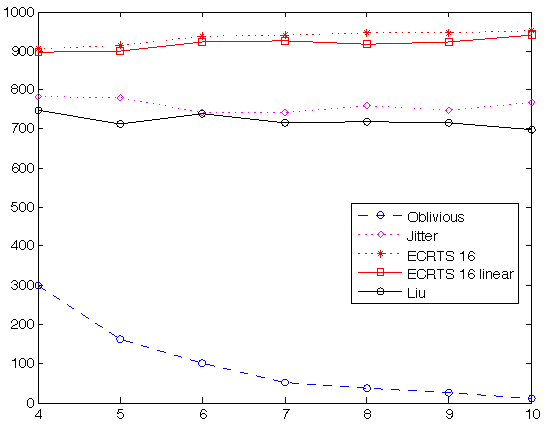
\includegraphics[width=0.4\textwidth]{../figures/experiments/varyingn_smin=5_smax=50_U=0_95_T=100-10000_1000runs_croped.pdf}}
  \subfloat[Varying $r_{\max}$, $U'=1$, $n=8$, $r_{\min} = 0.05$]{\label{fig:plot2} 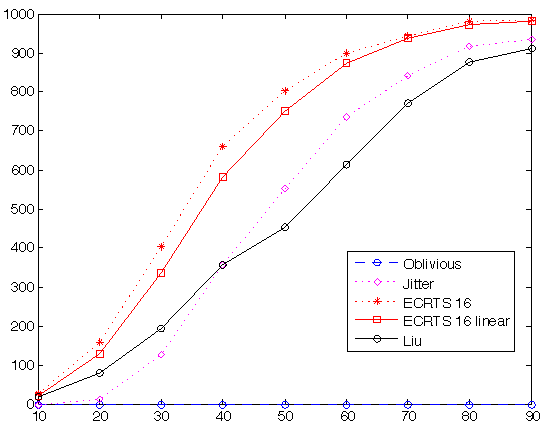
\includegraphics[width=0.4\textwidth]{../figures/experiments/varyingSmax_smin=5_U=1_n=8_T=100-10000_1000runs_croped.pdf}}\\ 
  \subfloat[Varying $U'$, $n=8$, $r_{\min} = 0.05$, $r_{\max} = 0.5$]{\label{fig:plot3} 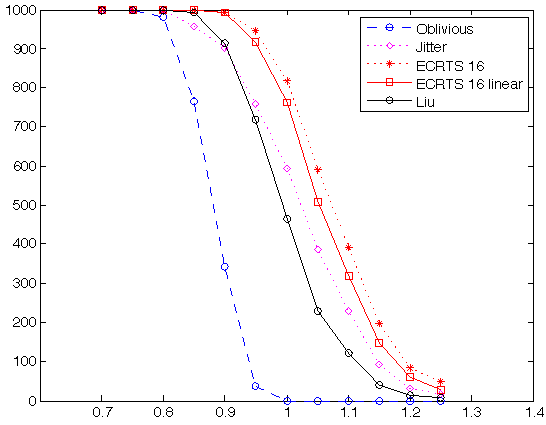
\includegraphics[width=0.4\textwidth]{../figures/experiments/varyingU_smin=5_smax=50_n=8_T=100-10000_1000runs_croped.pdf}}
  \subfloat[Varying $U'$, $n=8$, $r_{\min} = 0.5$, $r_{\max} = 0.9$]{\label{fig:plot4} 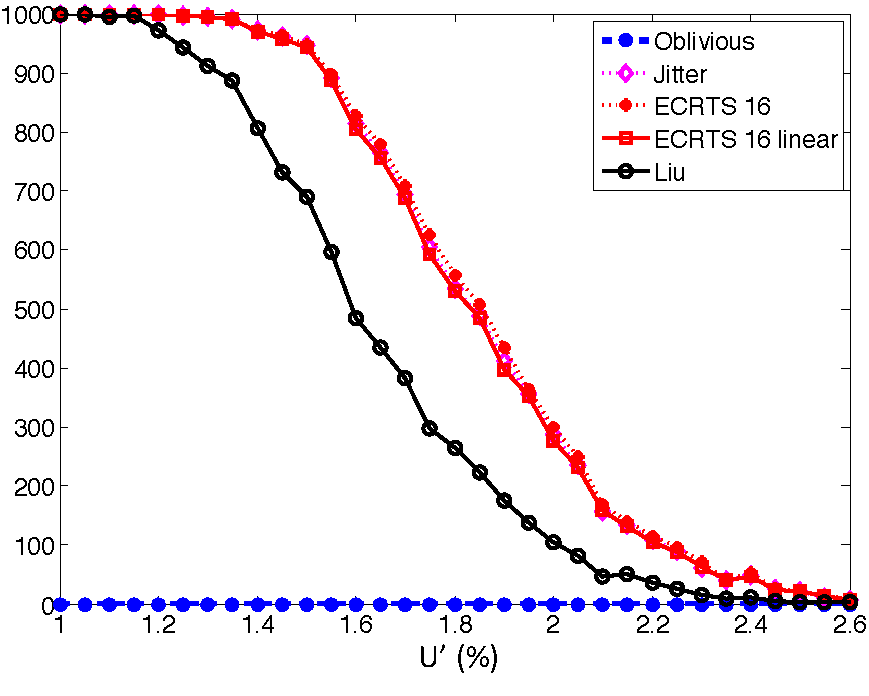
\includegraphics[width=0.4\textwidth]{../figures/experiments/varyingU_smin=50_smax=90_n=8_T=100-10000_1000runs_croped.pdf}} 
  \caption{Number of schedulable task sets over $1000$ randomly generated task sets.}
  \label{fig:exp}
\end{figure*}

Each point in the plots of Figure~\ref{fig:exp} represents the number of task sets that were deemed schedulable by the respective algorithm over $1000$ different experiments.

Four different types of experiments are reported in this paper. The first one is presented in Figure~\ref{fig:plot1}. It presents the evolution of the number of task sets deemed schedulable when the number of self-suspending tasks increases. The number of tasks $n$ is varied from $4$ to $10$ for a total modified utilization $U'$ of $0.95$. As can be seen in Figure~\ref{fig:plot1}, at the exception of the suspension oblivious analysis, the performances of the tests are barely influenced by the number of tasks. In fact, the number of task sets found schedulable by the test of Corollary~\ref{corollary:general-framework} and the linear test of Section~\ref{sec:linear-approximation} slightly increases with the number of tasks. It is the opposite behavior than the suspension oblivious approach. One can already conclude from this plot that the tests developed in this paper perform way better than the state-of-the-art. Furthermore, the difference between the performances of the complete test of Corollary~\ref{corollary:general-framework} and its linear version are quite small, thereby making the linear test a practical and useful analysis.

The second experiment is presented in Figure~\ref{fig:plot2} and shows the evolution of the performances of the tests with respect to the length of the total suspension time of a task when the total modified utilization $U'$ and the number of tasks are kept constant. The value of $r_{\max}$ is then varied from $10\%$ to $90\%$, hence increasing the number of tasks with high suspension times. The value $r_{\min}$ is kept constant at $5\%$, so as to keep a certain diversity in the suspension behavior of each task. As expected, the suspension oblivious approach does not accept any task set since the total modified utilization is equal to $100\%$. For the other tests however, the number of schedulable task sets increases when the suspension times become larger. Indeed, the actual workload, which accounts only for the WCET $C_i$, decreases when $S_i$ increases. Again, one can see the improvement of the tests of this paper over the state-of-the-art. Interestingly, one can also witnesses the incomparability of the jitter based and the blocking based schedulability tests. The jitter based test performs better for large blocking times while the blocking based test has better results for lower blocking times.

The last two plots (Figures~\ref{fig:plot3} and~\ref{fig:plot4}), present the results obtained when the total modified utilization increases but the distribution of suspension times and the number of tasks remain identical. As expected, the number of schedulable task sets decreases when the utilization increases. Again, the incomparability of the jitter- and blocking-based tests can be seen. The test based on blocking usually performs better for lower utilizations. The improvement of Corollary~\ref{corollary:general-framework} over the state-of-the-art is still high when suspension times are in average smaller than the execution times of the tasks (see Figures~\ref{fig:plot3}). However, when the suspension time becomes larger than the execution time of the task (see Figures~\ref{fig:plot4}), the release jitter-based test performs almost as well as Corollary~\ref{corollary:general-framework}.



.\\
.\\
.\\
.\\
.\\
.\\
.\\
.\\
.\\
.\\
.\\
.\\
.\\
.\\
.





\noindent{\bf Acknowledgement:} This paper is supported by DFG, as part of the Collaborative Research Center SFB876 (http://sfb876.tu-dortmund.de/). This work was also partially supported by National Funds through FCT/MEC (Portuguese Foundation for Science and Technology) and co-financed by ERDF (European Regional Development Fund) under the PT2020 Partnership, within project UID/CEC/04234/2013 (CISTER); also by FCT/MEC and the EU ARTEMIS JU within project(s) ARTEMIS/0003/2012 - JU grant nr. 333053 (CONCERTO) and ARTEMIS/0001/2013 - JU grant nr. 621429 (EMC2).

\bibliography{../bibliography/biblio-summary,../bibliography/biblio}{}

\end{document}
